\documentclass[12pt]{article}
\usepackage[letterpaper]{geometry}
\usepackage{indentfirst}
\usepackage{tabularx}
\usepackage{graphicx}
\usepackage{multirow}
\usepackage{amsmath}
\usepackage{siunitx}
\setlength{\parindent}{2em}
\geometry{left=1.0in, bottom=1.5in, left=1.0in, right=1.0in}
\begin{document}
    \thispagestyle{empty}
	\renewcommand\thesection{\Roman{section}}
    \begin{titlepage}

\newcommand{\HRule}{\rule{\linewidth}{0.5mm}}

\center

\textsc{\LARGE UM - SJTU Joint Institute}\\[1cm]
\textsc{\Large Physics Laboratory I}\\[0.5cm]
\textsc{\large VP141}\\[0.5cm]

\HRule \\[0.4cm]
{
    \bfseries
    {\huge Exercise II}\\[0.3cm]
    {\large Measurement of Fluid Viscosity}\\[0.2cm]
    \HRule \\[1.5cm]
}

\begin{minipage}{0.6\textwidth}

\large
\emph{Name:}\\
Tianyi \textsc{Ge} \\

\emph{Student Number:}\\
516370910168 \\

\emph{Group:}\\
17\\

\emph{Instructor:}\\
Prof. Mateusz \textsc{Krzyzosiak}

\end{minipage}\\[3.5cm]

{\large \today}\\[2cm]

\vfill

\end{titlepage}
    \newpage
    \section{Introduction}
    \subsection{objective}
        The objective of the exercise is to measure the fluid viscosity,
        which is one of the most important properties of fluids, determining the
        fluid’s flow, by using a common and simple method called Stokes' method.
    \subsection{Theoretical Background}
        When an object moves in a fluid, its motion is hindered by a drag force acting in the opposite 
        direction of the movement of object.Also, the magnitude of the drag force is related to serval 
        components such as, the shape, speed of the object as well as the internal friction in the fluid.
        Usually, we use coefficient $\eta$ to quantify the internal friction in the fluid, and the $\eta$
        is konwn as the viscosity coefficient. The drag force of a spherical object with radius R moving at 
        speed v in an infinite volume of a liquid is given by,
        \begin{equation} \label{F1}
        F_1=6\pi\eta vR
        \end{equation}
        And the buoyancy force is,
        $$F_3=\frac{4}{3}\pi R^3\rho_1g$$   
        Where $\rho$ is the density of fluid and $g$ is the acceleration due to gravity.The weight of the object is
        $$F_3=\frac{4}{3}\pi R^3\rho_2g$$
        After sometime, the ball will achieve equilibrum speed when the three force balance each other,
        \begin{equation} \label{Balance}
            F_1+F_2=F_3.
        \end{equation}
        Together with the euation 1, we get,
        \begin{equation}\label{3}
                    \eta=\frac{2}{9}gR^2\frac{\rho_2-\rho_1}{v_t}.
        \end{equation}
        Because of the constant velocity, the $\eta$ can also be written as
        \begin{equation} \label{eta}
            \eta=\frac{2}{9}gR^2\frac{(\rho_2-\rho_1)t}{s},
        \end{equation}
        where $s$ is the distance travled in time $t$ with reaching the terminal speed.\\
        Since the volume of the fluid is not infinite,the results are affected by some boundary effect due to the presence of the container.Therefore the formula for the crrected magnitude is giben by,
        $$F_1=6\pi\eta vR(1+2.4\frac{R}{R_c})$$
        Where $R_c$ is the radius of the infinitely long cylindrical container.Consequently, we get,
        \begin{equation} \label{eta2}
                \eta=\frac{2}{9}gR^2\frac{(\rho_2-\rho_1)t}{s}\frac{1}{1+2.4\frac{R}{R_c}}.
        \end{equation}
    \section{Apparatus and Measurement procedure}
    \subsection{Experimental Setup}
    This exercise requires a Stokes' viscosity measurement device  with castor oil and some small metal balls. There are also a number of measurement devices including micrometer, calliper, densimeter, electronic scales, stopwatch, and thermometer.
    \begin{figure}[htbp]
        \centering
        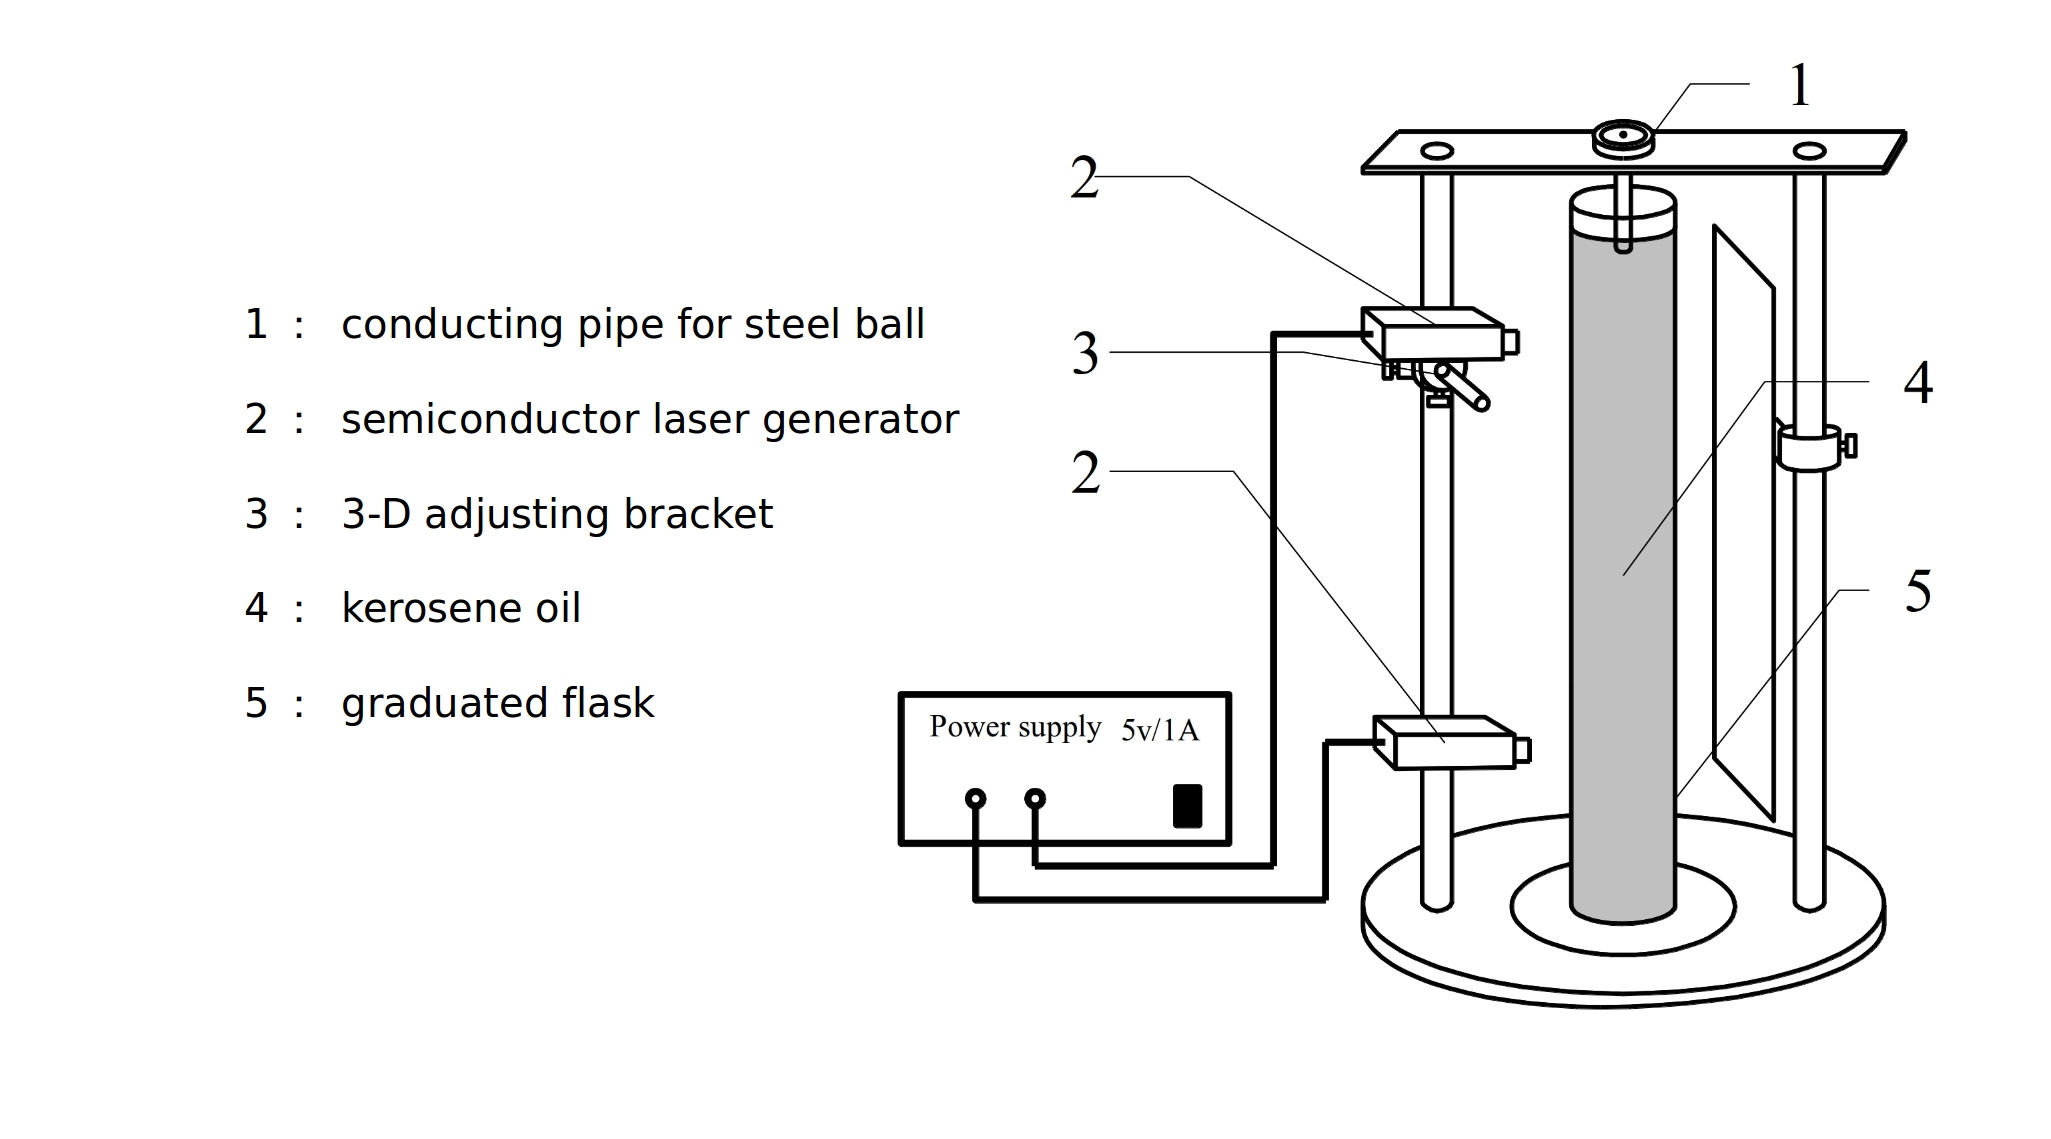
\includegraphics[width=0.8\linewidth]{1.png}
        \caption{Stokes’ viscosity measurement apparatus}
        \label{apparatus}
    \end{figure}
    \subsection{Measurement}
        \subsubsection{Adjustment of the Stokes' viscosity measurement device}
            \begin{enumerate}
                \item Make the plumb aiming at the center of the base by adjusting the knobs beneath the base.
                \item Turn on the two lasers and make the beams parallel and aim at the plumb line.
                \item Remove the plumb and place the flask with castor oil at the center of the base.
                \item Place the guiding pipe on the top of the device.
                \item Put a metal ball into it and check whether the ball can block the beams. If not, repeat. 
            \end{enumerate}
        \subsubsection{Measurement of the (constant) velocity of a falling ball}
            \begin{enumerate}
                \item Measure the vertical distance $s$ between the two laser beams at least three times.
                \item Put a metal ball into the guiding pipe. Record the time it travels between the two beams for at least six times.
            \end{enumerate}
        \subsubsection{Measurement of the ball density $\rho_2$}
            \begin{enumerate}
                \item Use electronic scales to measure the mass of 40 metal balls. Calculate the average.
                \item Use a micrometer to measure the diameter of the ball for ten times.
                \item Calculate the density $\rho_2$.
            \end{enumerate}
        \subsubsection{Other measurements}
            Measure of the density $\rho_1$ of the castor oil by using the provided densimeter (one
            measurement). Use a calliper to measure the inner diameter D of the graduated
            flask for six times. Read the ambient temperature from the thermometer placed in
            the lab.  
        \section{Results}
        \subsection{Measurement of the Distance}
        \begin{table}[h]
        \centering
        \begin{tabular}{|c|c|c|c|}
            \hline
            \multicolumn{4}{|c|}{$Distance\ S\ [\times10^{-3}m] \pm\ 0.10\ [\times10^{-3}m]$}\\
            \hline
            $S_1$ &110.0 & 263.0 &153\\
            \hline
            $S_2$ &140.0 &292.0 &152\\
            \hline
            $S_3$ &111.0 &264.5 &153.5\\     
            \hline
        \end{tabular}\\
        \caption{Distance measurement data}
        \label{distance}
        \end{table}
        The average value of the vertical distance of two beams is hence calculated by,
        $$\bar{S}=\frac{1}{3}\sum_{i=1}^{3}S_i=(152.8\pm1.55)\times10^{-3}m$$
        \subsection{Measurement of the Time}
        \begin{table}[htbp]
        \centering
        \begin{tabular}{|c|c|}
            \hline
            \multicolumn{2}{|c|}{Measurement $Time\ t\ [s] \pm\ 0.01\ [s]$}\\
            \hline
            $t_1$ & 6.97\\
            \hline
            $t_2$ & 7.12\\
            \hline
            $t_3$ & 7.28\\
            \hline
            $t_4$ & 7.35\\
            \hline
            $t_5$ & 6.94\\
            \hline
            $t_6$ & 7.00\\
            \hline
        \end{tabular}\\
        \caption{Time measurement data}
        \label{time}
    \end{table}
    The average value of the time is given as
    \[
        \bar{t}=\frac{1}{6}\sum_{i=1}^{6}t_i=7.11\pm 0.157s
    \]
    \subsection{Diameter of ball}
        \begin{table}[htbp]
        \centering
        \begin{tabular}{|c|c|c|c|}
            \hline
            \multicolumn{4}{|c|}{ $Diameters\ d[\times10^{-3}m] \pm 0.004[\times10^{-3}m]$}\\
            \hline
            $d_1$ &1.945 &$d_6$ &1.955\\
            \hline
            $d_2$ &1.945 &$d_7$ &1.940\\
            \hline
            $d_3$ &1.950 &$d_8$ &1.940\\
            \hline
            $d_4$ &1.955 &$d_9$ &1.950\\
            \hline
            $d_5$ &1.950 &$d_{10}$ &1.935\\         
            \hline
        \end{tabular}\\
        \caption{Measurement data for diameters of the balls}
        \label{balldiameter}
    \end{table}     
    With the initial reading, $d_0 = -0.040 mm$
    The average value of the diameter of a ball is hence calculated as
    \[
        \bar{d}=\frac{1}{10}\sum_{i=1}^{10}d_i=(1.986\pm )\times10^{-3}m
    \]
    \subsection{Inner Diameter of the Flask}
    \begin{table}[htbp]
        \centering
        \begin{tabular}{|c|c|}
            \hline
            \multicolumn{2}{|c|}{$Diameters\ D[\times10^{-3}m] \pm 0.02[\times10^{-3}m]$}\\
            \hline
            $D_1$ & 61.70\\
            \hline
            $D_2$ & 61.78\\
            \hline
            $D_3$ & 61.68\\
            \hline
            $D_4$ & 61.70\\
            \hline
            $D_5$ & 61.64\\
            \hline
            $D_6$ & 61.68\\ 
            \hline          
        \end{tabular}\\
        \caption{Measurement data for the inner diameter of the flask}
        \label{innerdiameter}
    \end{table}
    \newpage
    The average value of the inner diameter of the flask is hence calculated 
    \[
        \bar{D}=\frac{1}{6}\sum_{i=1}^{10}D_i=(61.69\pm0.105)\times10^{-3}\ m
    \]
    \subsection{Other Physicals Quantifies}
    \begin{table}[htbp]
        \centering
        \begin{tabular}{ll}
            \hline\hline
            Density of the castor oil & $\rho_1=0.956\pm 0.001g/cm^3$\\
            \hline
            Mass of 40 metal balls & $m=1.359\pm 0.001\times10^{-3}kg$\\
            \hline      
            Temperature in the lab & $T=26\pm \SI{2}{\degreeCelsius}$\\
            \hline
            Acceleration due to gravity in the lab & $g=9.794m/s^2$\\        
            \hline\hline
        \end{tabular}\\
        \caption{Values of other physical quantities}
        \label{other}
    \end{table}
    \section{Calculation and Uncertainy Analysis}
        For a single measurement of the experiment setup, the uncertainty of the measurement instruments are
        \begin{table}[h]
        \centering
        \begin{tabularx}{\textwidth}{|c|c|c|c|c|c|c|}
            \hline
            Distance  & Time & Diameter of Ball& Diameter of Flask &Density & Mass & Temperature\\
            \hline
           0.1mm & 0.01s & 0.004mm &0.03mm &1$kg/m^3$ &0.001g &\SI{2}{\degreeCelsius} \\
            \hline
        \end{tabularx}
        \caption{Precision of the measurement instruments}
        \end{table}
    For the type-A uncertainty of the distance measurement, the standard  deviation of the average value is given by,
    $$s_X = \sqrt{\frac{1}{n-1}\sum_{i=1}^{n}(x_i - \bar{X})^2 }=0.6236mm$$
    and the type-A uncertainty is given by,
    $$\Delta_A = \frac{s_X\times t_{0.95}}{\sqrt{n}}$$
    where the $t_0.95$ is 4.3 for $n = 3$. Taking the data from Table 1, 
    $\Delta_A$ is calculated by,
    $$\Delta_A = \frac{0.6236\times4.3}{\sqrt{3}}=1.48mm$$ 
    $\Delta_B$ is equal to $0.1mm$.
    $$u = \sqrt{\Delta_A^2+\Delta_B^2}=\sqrt{1.548^2+0.1^2}\approx1.55mm$$
    Then, the relative uncertainty is,
    $$u_{r} = \frac{u}{\bar{x}}\times100\%=1.0\%$$
    We thus achieve $$S = (152.8 \pm 1.55)\times10^{-3}m$$
    \begin{table}[h]
    \centering
    \begin{tabularx}{\textwidth}{|p{5cm}|X|p{2cm}|p{2cm}|p{1.8cm}|X|}
        \hline
         &Value &$s_X$ & $\Delta_{A}$ & $u$ & $u_r$\\
        \hline
        Distance $[mm]$ &152.8 & 0.6236 &1.48 &1.55 &$1.0\%$\\
        Time $[s]$&7.11 &0.157 &0.165 &0.165 &$2.2\%$\\
        Diameter of Ball$[mm]$ &1.968 &$6.34\times10^{-3}$ &$4.53\times10^{-3}$ &$6\times10^{-3}$ &$0.304\%$\\
        Diameter of Flask$[mm]$&61.69 &0.0987 &0.103 &0.105 &$0.171\%$\\
        \hline
    \end{tabularx}
    \caption{The uncertainty}
    \end{table}
    \subsection{Uncertainy of density}
    Density of the mental balls can be found as,
    $$\rho_2 = \frac{m_o}{V} = \frac{6m_0}{\pi d^3}$$
    Where $m_0=\frac{1.359}{40}=0.03398\times10^{-3}kg$, and $d = 1.968 \times 10^{-3}m$, the desity is hence calculated by,
    $$\rho_2=\frac{6\times0.03398\times10^{-3}}{3.141593\times(1.968\times10^{-3})^3}=8.514\times10^{3}kg/m^3$$
    The uncertainty of the density is given by,
     \[
     u_{\rho_2}=\sqrt{(\frac{\partial\rho_2}{\partial m_0})^2(u_{m_0})^2+(\frac{\partial\rho_2}{\partial d})^2(u_d)^2}\\
    \]
    Where the partial derivatives is given by,
        \[
        \frac{\partial\rho_2}{\partial m_0}=\frac{6}{\pi d^3},\quad
        \frac{\partial\rho_2}{\partial d}=\frac{18m_0}{\pi d^4}
    \]
    Also, because the $m_{0} = \frac{M}{40}$, the uncertainty of $m_0$ is $\frac{\partial M}{\partial m_{0}}u_m=\frac{1\times0.001}{40}=2.5\times10^{-5}g$
    then,
    \[
    \begin{split}
        u_{\rho_2}&=\sqrt{(\frac{\partial\rho_2}{\partial m_0})^2(u_{m_0})^2+(\frac{\partial\rho_2}{\partial d})^2(u_d)^2}\\
        &=\sqrt{(\frac{6\times 0.00025\times10^{-3}}{3.1415926\times (1.968\times10^{-3})^3})^2+(\frac{18\times 0.03393\times10^{-3}\times 0.006\times10^{-3}}{3.14159\times (1.968\times10^{-3})^4})^2}\\
        &\approx 0.099 \times10^3kg/m^3.
    \end{split}
    \]
    The relative uncertainty is,
    $$u_{r\rho2} = \frac{u_{\rho_2}}{\bar{\rho_2}} \approx 1.16\% $$
    \subsection{Uncertainy of Viscosity Coefficient}
    Through the calculation above, the viscosity coefficient can hence be achieved as,
    \[
    \begin{split}
    \centering
        \eta&=\frac{2}{9}gR^2\frac{(\rho_2-\rho_1)t}{s}\frac{1}{1+2.4\frac{R}{R_c}}\\
            &=\frac{2}{9}\times 9.794\times 0.000984^2\times \frac{(8.514\times 10^3-0.956\times10^{3})\times 7.11}{0.153}\times \frac{1}{1+2.4\times \frac{0.000984}{0.030845}}\\
            &\approx 0.688\frac{kg}{m\cdot s}.
    \end{split}
    \]
    The uncertainty of the Viscosity Coefficient is given by the following formula,
    $$u_{\eta}=\sqrt{(\frac{\partial\eta}{\partial R})^2(u_R)^2+(\frac{\partial\eta}{\partial \rho_2})^2(u_{\rho_2})^2+(\frac{\partial\eta}{\partial \rho_1})^2(u_{\rho_1})^2+(\frac{\partial\eta}{\partial u_t})^2(u_t)^2+(\frac{\partial\eta}{\partial S})^2(u_S)^2+(\frac{\partial\eta}{\partial u_{R_c}})^2(u_{R_c})^2}$$
    And the partial derivatives is found as,
    \begin{equation}
            \frac{\partial\eta}{\partial R}=- \frac{R Rc g t}{s \left(2.4 R + Rc\right)^{2}} \left(\frac{8}{15} R + \frac{4}{9}Rc\right) \left(\rho_{1} - \rho_{2}\right)
    \end{equation}
    \begin{equation}
            \frac{\partial\eta}{\partial \rho_2} = \frac{2 R^{2} R_c g t}{9s \left(2.4 R + R_c\right)}
    \end{equation}
    \begin{equation}
            \frac{\partial\eta}{\partial \rho_1} = - \frac{2 R^{2} R_c g t}{9s \left(2.4 R + R_c\right)}
    \end{equation}
    \begin{equation}
            \frac{\partial\eta}{\partial t} = - \frac{2 R^{2} Rc g \left(\rho_{1} - \rho_{2}\right)}{9 s \left(2.4 R + Rc\right)}
    \end{equation}
    \begin{equation}
            \frac{\partial\eta}{\partial S} = \frac{2 R^{2} R_c g t \left(\rho_{1} - \rho_{2}\right)}{9 s^{2} \left(2.4 R + R_c\right)}
    \end{equation}
    \begin{equation}
            \frac{\partial\eta}{\partial R_c} = - \frac{8 R^{3} g t \left(p_{1} - p_{2}\right)}{15 s \left(2.4 R + Rc\right)^{2}}
    \end{equation}
    By the equation through (6) to (11), the uncertainty is approxmately $0.03kg/m s$.
    The relative uncertainty is approxmately $3.8\%$\\
    Hence the experimentally $\eta$ is
    $$\eta = 0.688 \pm 0.03 kg/m s$$
\section{Conclusion and Discussion}
    In this experiment, by using  Stokes' method, the experimentally found $\eta$ of castor oil in the environment of $\SI{26}{\degreeCelsius}, 1\ atm$ is
        $$\eta=0.688\pm 0.03 kg/m s$$
        $$\quad u_{r_{\eta}}=3.8\%$$
    In this experiment, I find the mental ball is so small that it's hard to conver the lase, and I have to measure much more than 6 times and throw a couple of balls into the fluid. Also, it's hard to comfirm whether the two beams are parallel. When I measure the time, I always have to react some time before press the stopwatch when the laser is cover, and this will leads to uncertainty. If the equipment ensure the two beams is parallel and fixed, and the time is measured by computer when the beams is blocked, the results will be much more accurate.
\begin{thebibliography}{99}
    \bibitem{foo2} \textsc{Qin} Tian, \textsc{Feng} Yaming, Mateusz \textsc{Krzyzosiak} Physics Laboratory Vp141 Exercise 2 Measurement of Fluid Viscosity.
\end{thebibliography}
\end{document}